\scanpage{47}

\uline{Proposition} Soit $k$ un corps, $n$ un entier. Conditions équivalentes

a) $H^i(k,G)=0$ pour $i>n$ et tout groupe alg. comm. $G$ déf/$k$

b) $H^i(k,\Gamma\deleted{\unsure{G}})=0$ \hfill \uline{fini} $\Gamma$ déf/$k$

\deleted{\unsure{c)}} b') $H^i(k,\unsure{\Gamma|F})=0$ pour $i>n$ et tout \deleted{groupe vectoriel} \inserted{groupe \inserted{(fini)} $\Gamma$ qui est un espace} vectoriel sur un corps $\mathbb Z/l$, dans lequel $\unsure{\mathfrak g_k}$ opère (avec noyau ouvert) irréductiblement
\margin{$b,b'$ \unsure{sont tjrs} vérifiés $(\unsure{n>0|n\geq0})$ si $\Gamma$ est un $p$-groupe \deleted{\illegible{1}}}

c) $H^i(k,G)={}$ pour $i>n$ et tout groupe alg. comm. $G$ déf/$k$ \deleted{connexe affine} devenant isomorphe à un groupe \deleted{$\unsure{(G_m)^n}$} $(G_m)^n$ sur la clôture galoisienne de $k$

c') $H^i(k,G)$ \deleted{$\unsure{=0}$} pour $i>n$, chaque fois que $G$ est le groupe \inserted{\unsure{(comm.)}} des éléments inversibles d'une algèbre \deleted{\unsure{semi-simple}} \inserted{séparable} déf/$k$

\uuline{Démonstration}
\diagram{\begin{tikzcd}[column sep=small,row sep=small]
&a\arrow[dl,Rightarrow]\arrow[dr,Rightarrow]&\\
b\arrow[d,Rightarrow]&&c\arrow[d,phantom,"\deleted{\unsure{\Downarrow}}" description]\\
b'&&\unsure{c'|a'}
\end{tikzcd}}
est trivial. Nous prouverons $c\Rightarrow b'$ et $b'\Rightarrow\unsure{b\Rightarrow a}$ ce qui achèvera la démonstration

$b'\Rightarrow b)$ \deleted{En effet $b'\Rightarrow b$} comme on voit par un dévissage immédiat [\deleted{supposant} \inserted{se ramenant} d'abord à $\Gamma$ \deleted{\unsure{d'ordre}} \inserted{annulé} par $l^k$, puis en filtrant par $\Gamma\supset l\Gamma\supset l^2\Gamma\supset\cdots\supset l^{\unsure{n|k}}\Gamma=0$, au cas où $\Gamma$ est annulé par $l$ i.e. est un vectoriel sur $\mathbb Z/l$, puis enfin au cas irréductible].

$b\Rightarrow a$ \deleted{En effet, considérons le plus grand sous-groupe unipotent $G_1$ de $G$, (qui est défini sur $k$). Alors}
\figure{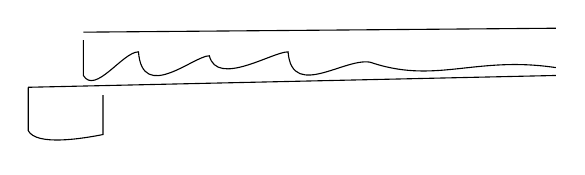
\begin{tikzpicture}[x=1cm,y=1cm]
\draw (0,0)--(6,.05);\draw (-.7,-.7)--(6,-.55);\draw (-.7,-.7)--(-.7,-1.25)..controls (-.6,-1.45) and (0,-1.35)..(.25,-1.3)--(.25,-.8);
\draw (0,-.1)--(0,-.55)..controls (.15,-.8) and (.5,-.25)..(.7,-.25)..controls (.75,-.9) and (1.4,-.3)..(1.6,-.3)..controls (1.7,-.7) and (2.4,-.25)..(2.6,-.25)..controls (2.65,-.9) and (3.4,-.25)..(3.7,-.4)..controls (4.5,-.65) and (5,-.3)..(6,-.45);
\end{tikzpicture}}
Supposons d'abord que le corps \deleted{\unsure{soit}} $k$ soit \uline{parfait}.
Soit alors $G_1$ le plus grand sous-groupe unipotent de $G$, on sait qu'il est \uline{défini sur $k$}, et on a de suite exacte
\diagram{\begin{tikzcd}[column sep=small]
0\arrow[r,dash]&G_1\arrow[r,dash]&G_{\deleted{\unsure{k}}}\arrow[r,dash]&G/G_1\arrow[r,dash]&0
\end{tikzcd}}
(déf/$k$)

\mspage{46}

